\chapter{Grammar school}

\begin{quote}
``... small number
of symbols and their grammar are enough to capture the huge
variety of equations...''
\end{quote}

The point of a variable is to replace it.  So in the formula 
$x(x+3)^2$ replacing $x$ for $7$ gives us $7(7+3)^2$.  
Yet even in the land of pure algebra where every symbol is variable it is absurd to
replace $+$ for $7$ to get $x(x73)^2$.   There is restraint in the substitution
of algebra built into what makes something an algebraic formula. When we pull 
on this thread we unravel an expansive relationship between free algebras and induction
and their role in computation.
% \medskip

% It is none other than grammar.

Consider how we know what to do when   
calculating $7(7+3)^2$.  For some of us a mnemonic springs to mind
(\emph{Please Excuse My Dear Aunt Sally}) or an acronym (PEMDAS).
These both unwind to tell us: Parenthesis Exponents Multiplication Division Addition Subtraction
in that order. This meandering thought process somehow elucidates how to read a formula. 
It gives the symbols complex structure that 
can be visualized with the following comic strip.
\begin{center}
    \begin{tikzpicture}[yscale=0.65]
        \node (A) at (0,0) {\begin{tikzpicture}[yscale=0.75]
        \node (f) at (0,0) {$7(7+3)^2$};
        \node[below of=f,scale=0.75] {$\times$};
        \node (x1) at (-1,-2) {$7$};
        \node (sqrt1) at (1,-2) {$(7+3)^{2}$}; 
        % \node[below of=sqrt1,scale=0.75] {$\circ$};
        \node (su) at (1.5,-3) {\textasciicircum $2$};
        \node (u) at (1,-4) {$7+3$};
        \node (x2) at (0,-6) {$7$};
        \node[below of=u,scale=0.75] {$+$};
        \node (three) at (2,-6) {$3$};
        % \node (x3) at (0,-8) {$x$};
        % \node (x4) at (2,-8) {$x$};
        % \node[below of=x2,scale=0.75] {$\times$};

        \draw[-] (f) -- (x1);
        \draw[-] (f) -- (sqrt1);
        % \draw[-] (sqrt1) -- (su);
        \draw[-] (sqrt1) -- (u);
        \draw[-] (u) -- (x2);
        \draw[-] (u) -- (three);
        % \draw[-] (x2) -- (x3);
        % \draw[-] (x2) -- (x4);

    \end{tikzpicture}};
    
    \node[right of=A,xshift=3cm] (B) {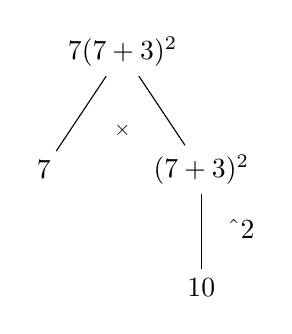
\begin{tikzpicture}[yscale=0.75]
        \node (f) at (0,0) {$7(7+3)^2$};
        \node[below of=f,scale=0.75] {$\times$};
        \node (x1) at (-1,-2) {$7$};
        \node (sqrt1) at (1,-2) {$(7+3)^{2}$}; 
        % \node[below of=sqrt1,scale=0.75] {$\circ$};
        \node (su) at (1.5,-3) {\textasciicircum $2$};
        \node (u) at (1,-4) {$10$};

        \draw[-] (f) -- (x1);
        \draw[-] (f) -- (sqrt1);
        % \draw[-] (sqrt1) -- (su);
        \draw[-] (sqrt1) -- (u);

    \end{tikzpicture}};
    
    \node[right of=B, xshift=3cm] (C) {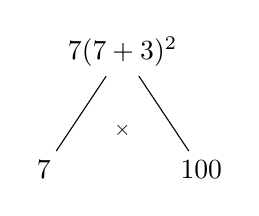
\begin{tikzpicture}[yscale=0.75]
        \node (f) at (0,0) {$7(7+3)^2$};
        \node[below of=f,scale=0.75] {$\times$};
        \node (x1) at (-1,-2) {$7$};
        \node (sqrt1) at (1,-2) {$100$}; 

        \draw[-] (f) -- (x1);
        \draw[-] (f) -- (sqrt1);

    \end{tikzpicture}};
    \node[right of=C,xshift=1cm] {$700$};

    \draw[thick] (A.north east) -- (A.south east);
    \draw[thick] (B.north east) -- (B.south east);
    \draw[thick] (C.north east) -- (C.south east);
\end{tikzpicture}
\end{center}
These step-by-step instructions start at the leaves $7$ and $3$ and join them as $7+3$ (computing $10$),
then the next step is to square (now $100$), then multiply by $7$, we reach $700$.
In hindsight, PEMDAS taught children a complicated form of induction.

\subsection{Induction \& Grammar}
You may have been taught induction through stories of falling 
dominos.  Good.  But what if induction was more like what we just did, climbing?
The domino illustration could bottle up the experience of climbing stairs.  
Now we climb trees and maybe mountains.
Setting up this induction was nothing more than a fragment of text but 
read through the lens of a grammar, e.g.\ PEMDAS, it came into a full form
as steps for recursion.

Parsing grammars in natural language is not always clarifying.  A simplistic
English grammar will often parse into cycles.
\begin{center}
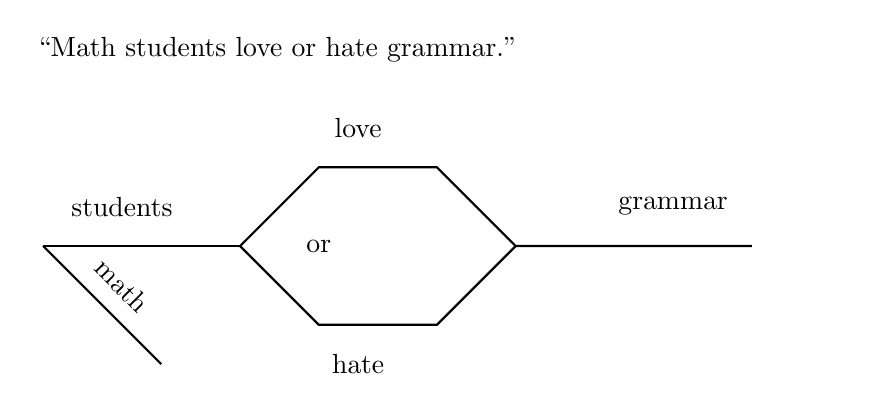
\begin{tikzpicture}
    \node[text width=4in] at (1,2) {``Math students love or hate grammar.''};
    \node at (-3,0) {students};
    \node[rotate=-45] at (-3,-1) {math};
    \node at (-0.5,-0.5) {or};
    \node at (0,1) {love};
    \node at (0,-2) {hate};
    \node at (4,0) {grammar};

    \draw[thick] (-4,-0.5) -- ++(2.5,0);
    \draw[thick] (-4,-0.5) -- ++(1.5,-1.5);
    \draw[thick] (-1.5,-0.5) -- ++(1,1) -- ++(1.5,0) -- ++(1,-1) -- ++(3,0);
    \draw[thick] (-1.5,-0.5) -- ++(1,-1) -- ++(1.5,0) -- ++(1,1);

\end{tikzpicture}
\end{center}
So our inductive climbs may one day need many routes, even go in cycles.
Fortunately, evaluating a formula has a precise algorithm without ambiguity. The
reason is that we had a rooted tree.  Trees have unique paths between any two
vertices. So if we start at the leaves we have a unique direction to reach the
root. 



\index{context-free}
That we got a tree in math formulas means we have a rather boring grammar, 
what Chompsky's \emph{Syntactic Structure} calls
\emph{context-free} grammars.\footnote{
    If an algebraist starts a talk with a story that ``...It was thought  all natural 
    languages were context-free until some obscure dialect in the alps or Africa was found...'', 
    then tune out until they return to equations.  
    Linguist never had such illusions. Even english is not context-free, read  James Higginbotham.} 
Don't be too disheartened.  Virtually every programming language has a 
context-free grammar and programs can communicate a lot of hefty ideas. 

\begin{quote}
    \textbf{Complex inductions can be specified by grammar.}
\end{quote}
